\documentclass[]{article}
\usepackage{lmodern}
\usepackage{amssymb,amsmath}
\usepackage{ifxetex,ifluatex}
\usepackage{fixltx2e} % provides \textsubscript
\ifnum 0\ifxetex 1\fi\ifluatex 1\fi=0 % if pdftex
  \usepackage[T1]{fontenc}
  \usepackage[utf8]{inputenc}
\else % if luatex or xelatex
  \ifxetex
    \usepackage{mathspec}
  \else
    \usepackage{fontspec}
  \fi
  \defaultfontfeatures{Ligatures=TeX,Scale=MatchLowercase}
\fi
% use upquote if available, for straight quotes in verbatim environments
\IfFileExists{upquote.sty}{\usepackage{upquote}}{}
% use microtype if available
\IfFileExists{microtype.sty}{%
\usepackage{microtype}
\UseMicrotypeSet[protrusion]{basicmath} % disable protrusion for tt fonts
}{}
\usepackage[unicode=true]{hyperref}
\hypersetup{
            pdfborder={0 0 0},
            breaklinks=true}
\urlstyle{same}  % don't use monospace font for urls
\usepackage{graphicx,grffile}
\makeatletter
\def\maxwidth{\ifdim\Gin@nat@width>\linewidth\linewidth\else\Gin@nat@width\fi}
\def\maxheight{\ifdim\Gin@nat@height>\textheight\textheight\else\Gin@nat@height\fi}
\makeatother
% Scale images if necessary, so that they will not overflow the page
% margins by default, and it is still possible to overwrite the defaults
% using explicit options in \includegraphics[width, height, ...]{}
\setkeys{Gin}{width=\maxwidth,height=\maxheight,keepaspectratio}
\IfFileExists{parskip.sty}{%
\usepackage{parskip}
}{% else
\setlength{\parindent}{0pt}
\setlength{\parskip}{6pt plus 2pt minus 1pt}
}
\setlength{\emergencystretch}{3em}  % prevent overfull lines
\providecommand{\tightlist}{%
  \setlength{\itemsep}{0pt}\setlength{\parskip}{0pt}}
\setcounter{secnumdepth}{0}
% Redefines (sub)paragraphs to behave more like sections
\ifx\paragraph\undefined\else
\let\oldparagraph\paragraph
\renewcommand{\paragraph}[1]{\oldparagraph{#1}\mbox{}}
\fi
\ifx\subparagraph\undefined\else
\let\oldsubparagraph\subparagraph
\renewcommand{\subparagraph}[1]{\oldsubparagraph{#1}\mbox{}}
\fi

% set default figure placement to htbp
\makeatletter
\def\fps@figure{htbp}
\makeatother


\date{}

\begin{document}

\emph{\textbf{Neoplasie dell'osso}}

Le neoplasie dell'osso e dei tessuti molli possono essere:

\begin{itemize}
\item
  \textbf{primitive}, cioè che iniziano e si sviluppano nel tessuto
  osteo-articolare
\item
  più frequentemente, \textbf{neoplasie secondarie} a metastasi, da
  tumori primitivi localizzati in altre regioni.
\end{itemize}

La patologia osteo-articolare primitiva tende ad interessare bambini ed
adolescenti, anche per questo sono tumori molto aggressivi e resistenti
alla terapia; per queste malattie è necessario un approccio
multidisciplinare.

\emph{Definizioni}

Alcune definizioni prima di trattare i tumori più frequenti:

\begin{itemize}
\item
  \textbf{IPERPLASIA:} accumulo di cellule dovuto o ad una
  proliferazione accelerata o ad una maturazione cellulare rallentata.
  Indotta da uno stimolo, scompare quando questo finisce. Solitamente il
  tessuto è costituito da una struttura cellulare ``organoide'' simile
  all'organo di origine.
\end{itemize}

\begin{quote}
Alcuni esempi: callo osseo esuberante attorno ad un focolaio di
frattura, miosite ossificante (calcificazione del tessuto muscolare,
iperplastico) per stravaso ematico a seguito di uno strappo muscolare
importante.
\end{quote}

\begin{itemize}
\item
  \textbf{AMARTOMA:} tumore benigno che deriva da AMARTIA, cioè un'isola
  di tessuto che durante lo sviluppo embrionale, fetale o infantile
  viene esclusa dall'organizzazione regionale. Questa porzione di
  tessuto può continuare a crescere dopo la nascita costituendo un
  amartoma.
\end{itemize}

\begin{quote}
Alcuni esempi: esostosi a livello della testa del perone, questo ``becco
osseo'' viene rimosso per evitare la compressione del nervo sciatico;
origina da abbozzi cartilaginei fetali che possono accrescersi durante
la vita extrauterina formando amartomi; angioma cutaneo (amartoma del
tessuto vascolare).
\end{quote}

\begin{itemize}
\item
  \textbf{TUMORE BENIGNO:} neoformazione a crescita autonoma ma più
  lenta del maligno, non presenta atipie cellulari e organizzazione
  cellulare ``organoide'', con cellule ben differenziate. Si tratta di
  un tumore ben delimitato, che cresce per continuità, non causa
  metastasi e non recidiva dopo exeresi.
\end{itemize}

\begin{quote}
Alcuni esempi: osteoma osteoide e tumore a cellule giganti.
\end{quote}

\begin{itemize}
\item
  \textbf{TUMORE MALIGNO:} può essere a basso, medio o alto grado a
  seconda dell'aggressività.
\end{itemize}

\begin{quote}
Si tratta sempre di neoformazioni a \emph{crescita autonoma}, con
velocità di crescita \emph{elevata}, le cellule sono \emph{atipiche} e
si organizzano in modo anarchico all'interno del tessuto di origine,
poco differenziate, possono causare metastasi e, se non completamente
asportate, possono recidivare localmente.

Alcuni esempi: osteosarcoma, tumore maligno del tessuto osseo con
prognosi altamente negativa; condrosarcoma, tumore maligno del tessuto
cartilagineo.
\end{quote}

Per classificare i tumori dell'osso primitivi è importante verificarne
la \textbf{localizzazione}:

\begin{itemize}
\item
  \textbf{INTRACORTICALE:} crescita all'interno della corticale ossea
\item
  \textbf{INTRAMIDOLLARE:} crescita all'interno dell'osso spugnoso
  sottocorticale
\item
  \textbf{PERIOSTALE:} crescita sulla superficie esterna dell'osso a
  livello diafisario, dove è presente periostio
\item
  \textbf{PAROSTALE} O IUXTACORTICALE: crescita sulla superficie esterna
  dell'osso, nelle metafisi dove non ho periostio. Lo sviluppo è nel
  punto di inserzione di capsula articolare, tendini e legamenti
\end{itemize}

Classificazione

In base al tipo di tessuto prodotto dal tumore:

\begin{itemize}
\item
  \begin{quote}
  tessuto osseo (neoplasie ossee osteoformative)
  \end{quote}

  \begin{itemize}
  \item
    \begin{quote}
    tessuto cartilagineo (neoplasie ossee condroformative)
    \end{quote}
  \item
    \begin{quote}
    tessuto vascolare
    \end{quote}
  \item
    \begin{quote}
    diversi tessuti molli (tessuto adiposo, fibroso, sinoviale)
    \end{quote}
  \end{itemize}
\end{itemize}

In base alle caratteristiche istologiche (importante per terapia e
prognosi), per definire il grado di malignità del tumore (basso, medio o
alto), si valuta:

\begin{itemize}
\item
  \begin{quote}
  cellularità
  \end{quote}
\end{itemize}

\begin{itemize}
\item
  \begin{quote}
  atipie
  \end{quote}
\end{itemize}

\begin{itemize}
\item
  \begin{quote}
  differenziazione
  \end{quote}
\item
  \begin{quote}
  encapsulazione (fattore prognostico positivo)
  \end{quote}
\end{itemize}

In base al tipo di cellule che compongono il tumore e al tessuto da cui
derivano:

\begin{itemize}
\item
  \begin{quote}
  fibroblasti e tessuto fibroso (fibroma, benigno, o fibrosarcoma,
  maligno)
  \end{quote}
\item
  \begin{quote}
  condroblasti o tessuto cartilagineo (condroma o --sarcoma)
  \end{quote}
\item
  \begin{quote}
  osteoblasti o tessuto osteoide (osteoma o --sarcoma)
  \end{quote}
\end{itemize}

Per curare le neoplasie ossee esistono dei centri regionali, il nostro
centro di riferimento è l'Istituto Rizzoli di Bologna.

Diagnosi

In caso di sospetto di neoplasia ossea, la diagnosi si basa su clinica,
esami strumentali e conferma bioptica. In alcuni casi, come osteoma
osteoide del calcagno, si ha certezza della diagnosi solo attraverso gli
esami strumentali, poiché questo tumore presenta caratteristiche
radiografiche preminenti.

In generale la diagnosi si basa su:

\emph{Anamnesi e caratteristiche cliniche del paziente}

\begin{itemize}
\item
  \textbf{età:} - tumore a cellule giganti: raro prima della pubertà

  \begin{itemize}
  \item
    \begin{quote}
    sarcoma di Ewing (si localizza soprattutto a livello del ginocchio):
    raro prima dei 5 anni e dopo i 30
    \end{quote}
  \item
    \begin{quote}
    condrosarcoma: raro nel bambino
    \end{quote}
  \end{itemize}
\item
  \textbf{velocità di accrescimento:} rapida nei tessuti maligni
\item
  \textbf{iperpiressia:} indicativa di \emph{sarcoma di Ewing}
\item
  \textbf{dolore:} - tipicità di alcuni tumori (osteoma osteoide causa
  un dolore tipicamente notturno)

  \begin{itemize}
  \item
    \begin{quote}
    dolore da \emph{frattura patologica} (improvviso ed acuto)
    \end{quote}
  \item
    \begin{quote}
    il \emph{condrosarcoma} è più doloroso del condroma
    \end{quote}
  \item
    \begin{quote}
    il \emph{sinovial sarcoma} è estremamente doloroso
    \end{quote}
  \end{itemize}
\end{itemize}

\begin{itemize}
\item
  \textbf{localizzazione:} - il \emph{condroma} è tipico nella mano a
  livello delle falangi

  \begin{itemize}
  \item
    \begin{quote}
    il \emph{tumore a cellule giganti} si localizza prevalentemente a
    livello delle metaepifisi delle ossa lunghe
    \end{quote}
  \end{itemize}
\end{itemize}

\emph{Radiografia (deve sempre essere eseguita)}

Ci permette di vedere:

\begin{itemize}
\item
  \begin{quote}
  \textbf{OSTEOLISI}, di cui si valuta:
  \end{quote}
\end{itemize}

\begin{itemize}
\item
  \emph{velocità di crescita}
\item
  Intaccamento delle corticali
\item
  presenza di osteogenesi reattiva
\item
  presenza di orletto sclerotico (osteoma osteoide).
\end{itemize}

\begin{quote}
- \textbf{OSTEOGENESI REATTIVA}

- \textbf{ESPANSIONE DEI TESSUTI MOLLI}

- \textbf{CALCIFICAZIONI NEI TESSUTI MOLLI}
\end{quote}

\emph{Angiografia}

Permette di valutare:

\begin{itemize}
\item
  la presenza di vascolarizzazione nel tumore (criterio prognostico
  negativo)
\item
  i rapporti con i vasi (importante prima dell'intervento valutare se un
  grosso vaso è stato intaccato o compresso)
\item
  i margini tumorali nei tre piani spaziali.
\end{itemize}

\emph{Scintigrafia con Tc 99}

Permette di:

\begin{itemize}
\item
  valutare se la neoplasia è captante il Tecnezio
\item
  visualizzare tutto lo scheletro e le neoformazioni non visibili all'
  Rx o localizzate a distanza (metastasi)
\item
  è un indice di \emph{quiescenza o} di \emph{attività} del tumore.
\item
  Rappresenta uno strumento utile nel post-operatorio per visualizzare
  possibili \emph{recidive} e anche nella valutazione della
  \emph{risposta} a radio e chemioterapia.
\end{itemize}

\emph{TAC}

Utile per valutare l'\textbf{estensione} del tumore e i
\textbf{rapporti} con vasi,visceri e strutture vascolari circostanti.

\emph{RMN}

Strumento utile per lo studio dei \textbf{tessuti molli} e del
\textbf{tessuto adiposo}, soprattutto dopo somministrazione di mezzo di
contrasto che ne aumenta la sensibilità.

\emph{Biopsia}

Fondamentale per \textbf{completare la diagnosi}.

Bisogna però considerare che si tratta di un compromesso fra il
desiderio di \emph{ottenere tessuto} per una diagnosi certa e il
\emph{rischio di spargere} inopportunamente \emph{cellule neoplastiche}
che potrebbero complicare la terapia.

Per ridurre il rischio di diffusione delle cellule neoplastiche, la via
di accesso di una biopsia incisionale dovrebbe essere localizzata lungo
la linea di incisione del trattamento chirurgico definitivo.

Esistono diverse tipologie di biopsia:

\begin{itemize}
\item
  \textbf{\emph{AGOBIOPSIA}:} aspirazione di poche cellule, con scarso
  rischio di contaminazione neoplastica, possibile solo per \emph{tumori
  molli} senza capsula ossea, ma a causa della scarsa raccolta può avere
  un'alta incidenza di falsi negativi.
\item
  \textbf{\emph{BIOPSIA CON TROCAR}} (aghi di dimensioni maggiori e
  cannulati)\textbf{:}utilizzata per i \emph{tessuti ossei}, si
  raccolgono ``losanghe'' di tessuto di 3- e, per questo motivo, vi è un
  maggiore rischio di contaminazione neoplastica ma al tempo stesso una
  minore incidenza di falsi negativi.
\item
  \textbf{\emph{BIOPSIA INCISIONALE}:} eseguita se le precedenti non
  hanno dato risultati certi e nei casi in cui sia richiesto molto
  tessuto.
\end{itemize}

TRATTAMENTO

Può essere di tre tipi:

\begin{enumerate}
\def\labelenumi{\arabic{enumi}.}
\item
  \textbf{ASTENSIONISTICO:} valuto nel tempo come evolvono certi tumori
  benigni o pseudo tumori, che possono anche autolimitarsi nel tempo
\item
  \textbf{CHIRURGICO} con o senza adiuvanti (fenolo,alcol), utilizzati
  per distruggere le cellule tumorali, ed innesti ossei: si può eseguire
  un'escissione più o meno ampia
\item
  \textbf{CHEMIO} o \textbf{RADIOTERAPIA:}
\end{enumerate}

\begin{itemize}
\item
  \emph{neoadiuvanti}, ovvero prima del trattamento chirurgico.
  Permettono la riduzione delle dimensioni della massa tumorale.
\item
  \emph{adiuvanti}, cioè post-intervento. Per rimuovere le cellule
  neoplastiche rimaste.
\end{itemize}

\emph{Trattamento chirurgico}

L'\textbf{escissione} può essere più o meno ampia a seconda della
localizzazione dei margini chirurgici, cioè dalla quantità e qualità dei
tessuti che ricoprono il tumore dopo la sua asportazione.

Esistono varie tipologie di asportazione:

\begin{itemize}
\item
  \textbf{INTRALESIONALE}, quando il tumore è ``sbucciato'' della sua
  capsula o pseudo capsula (quindi viene enucleato) o interrotto anche
  in una minima area della sua superficie; per il rischio di lasciare
  cellule tumorali in situ viene utilizzata solo per \emph{neoplasie a
  bassa malignità} (osteoma osteoide, tumore a cellule giganti, cisti
  ossee) e si fa uso di adiuvanti come fenolo o alcol durante
  l'intervento.
\end{itemize}

\begin{quote}
All'interno delle cisti viene addirittura inserito cemento.
\end{quote}

\begin{itemize}
\item
  \textbf{MARGINALE}, quando il tumore viene rimosso in blocco
  completamente ricoperto dalla sua capsula o pseudo capsula
\item
  \textbf{AMPIA}, quando il tumore è rimosso in blocco e completamente
  ricoperto da uno strato continuo di tessuto normale
\item
  \textbf{RADICALE}, quando il tumore è rimosso in blocco con l'intero
  compartimento anatomico di origine circondato dalle sue naturali
  barriere (ad esempio se si rimuove il femore in toto).
\end{itemize}

TUMORI BENIGNI OSTEOFORMATORI

\emph{OSTEOMA OSTEOIDE}

Si tratta di una piccola e dolente neoformazione costituita da
\textbf{tessuto osteoide}, osso intrecciato, e circondato da un piccolo
e dolente \emph{alone reattivo}, cioè un orletto sclerotico reattivo
attorno alla lesione.

\begin{itemize}
\item
  \textbf{\emph{Epidemiologia}}
\end{itemize}

Colpisce i giovani fra i 5 e i 30 anni, con un rapporto M/F 2,5/1

\begin{itemize}
\item
  \textbf{\emph{Localizzazione}}
\end{itemize}

Di solito colpisce la zona diafiso-metafisaria corticale dello scheletro
appendicolare

\begin{itemize}
\item
  \textbf{\emph{Clinica}}
\end{itemize}

\begin{quote}
Si tratta di un tumore molto vascolarizzato che causa dolore notturno
sensibile all'acido acetilsalicilico, perché è un tumore che produce al
suo interno un'ingente quantità di prostaglandine e il farmaco va a
bloccare questa produzione.
\end{quote}

\begin{itemize}
\item
  \textbf{\emph{Diagnosi strumentale}}
\end{itemize}

\begin{quote}
L'osteoma osteoide è visibile alla radiografia con due segni specifici,
cioè la presenza di un'osteolisi a ``nidus'' e attorno ad essa la
presenza di un orletto sclerotico.
\end{quote}

La scintigrafia ossea è positiva con un quadro di ``faro nella nebbia''

Un'ulteriore indagine può essere rappresentata dalla TAC con m.d.c.

\begin{itemize}
\item
  \textbf{\emph{Trattamento}}
\end{itemize}

Asportazione chirurgica della neoformazione

\begin{quote}
Il tessuto patologico ha un aspetto molto diverso rispetto all'osso
normale, che è giallastro, perché si presenta di colore rossastro dovuto
all'ingente vascolarizzazione.

Nelle localizzazioni molto profonde come a livello del collo femorale o
a livello vertebrale si possono eseguire degli interventi di radiologia
interventistica, che vanno a distruggere l'osteoma osteoide con le
radiofrequenze.
\end{quote}

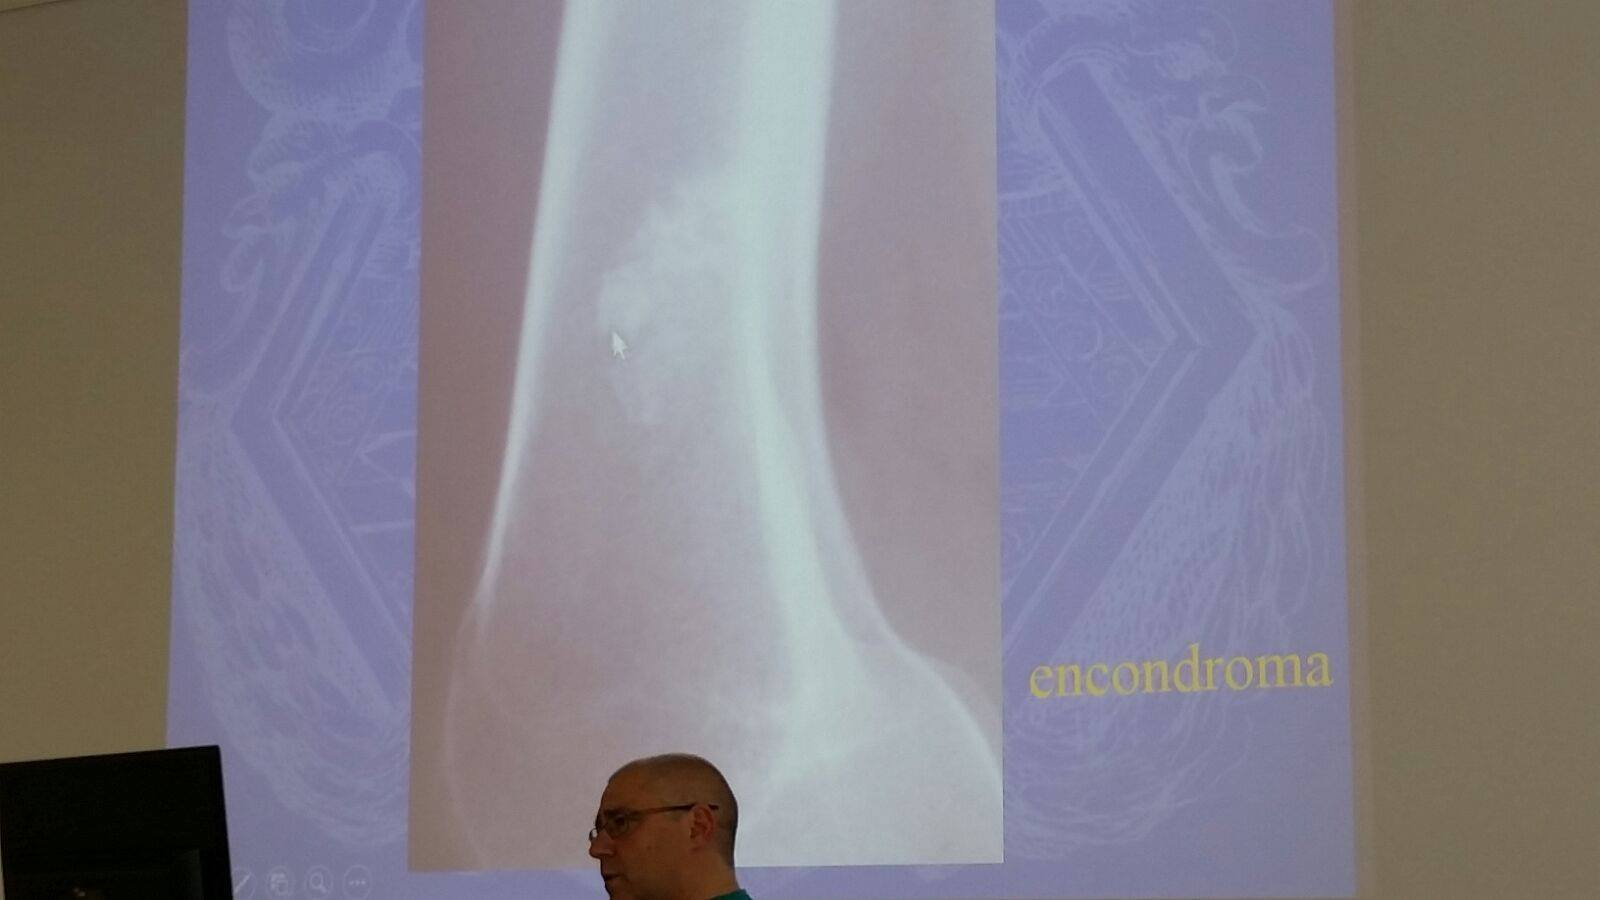
\includegraphics[width=2.11597in,height=2.59306in]{media/image1.jpeg}

\begin{quote}
In questa immagine radiologica si può notare il tipico aspetto a
``nidus'' dell'osteoma osteoide con la parte biancastra attorno che
rappresenta l'orletto sclerotico.
\end{quote}

TUMORI MALIGNI OSTEOFORMATORI

\emph{OSTEOSARCOMA}

Tumore maligno costituito da \textbf{cellule mesenchimali} che producono
tessuto osteoide e \textbf{osseo immaturo}.

\begin{itemize}
\item
  \textbf{\emph{Epidemiologia}}
\end{itemize}

\begin{quote}
Colpisce i giovani, generalmente fra i 10 e i 20 anni; M/F 2/1; si
tratta del secondo tumore osseo maligno per frequenza dopo il
condrosarcoma
\end{quote}

\begin{itemize}
\item
  \textbf{\emph{Localizzazione}}
\end{itemize}

A livello diafiso-metafisario delle ossa lunghe (70\% ginocchio e
spalla)

\begin{itemize}
\item
  \textbf{\emph{Clinica}}
\end{itemize}

\begin{quote}
Compare dolore e ci può essere una tumefazione calda, limitazione del
movimento articolare e febbre. Essendo un tumore che determina
osteolisi, vi sarà un aumento tipico di fosfatasi alcalina e LDH.
\end{quote}

\begin{itemize}
\item
  \textbf{\emph{Diagnosi strumentale}}
\end{itemize}

\begin{quote}
Dal punto di vista radiologico si vede un'evoluzione della lesione: il
tumore inizialmente è intraosseo, poi tende a diventare extraosseo.
\end{quote}

La scintigrafia ossea è positiva, come TAC e RMN.

\begin{quote}
Caratteristiche radiologiche peculiari: osteolisi ed addensamenti con
reazione periostale ``a sole nascente''
\end{quote}

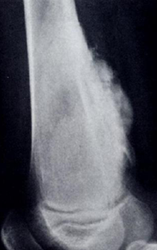
\includegraphics[width=2.18611in,height=3.47708in]{media/image2.png}

\begin{itemize}
\item
  \textbf{\emph{Trattamento}}
\end{itemize}

\begin{quote}
Solitamente il trattamento è \textbf{doppio}:
\end{quote}

\begin{enumerate}
\def\labelenumi{\arabic{enumi}.}
\item
  \emph{chemioterapia pre-operatoria}, 2 mesi prima dell'asportazione,
  per ridurre le dimensioni del tumore
\item
  \emph{escissione radicale} della neoplasia.
\end{enumerate}

\begin{quote}
A seguito dell'asportazione possono essere posizionate delle
\textbf{protesi tumorali specifiche} (ad esempio a livello del
ginocchio), molto spesso fatte su misura per il paziente, che vanno a
sostituire gran parte o totalmente femore e tibia.
\end{quote}

\end{document}
